\documentclass[a4paper,11pt]{article}

\usepackage[english]{babel}
\usepackage[utf8]{inputenc}
\usepackage[vmargin=3.5cm,hmargin=2cm]{geometry}
\usepackage{graphicx}
\usepackage{caption}
\usepackage{subcaption}
\usepackage{amsmath}
\usepackage{mathtools}
\usepackage{fancyhdr}
\usepackage{listings}

\setlength{\footskip}{0cm}
\setlength\parindent{0pt}
\addtolength{\footskip}{0.8cm}
\addtolength{\headsep}{-.5cm}

\title{\bfseries Lab 5: \\ An Initial Exposure to mmWave Radar Sensing\\}
\date{}

\lfoot{}
\cfoot{}
\rfoot{\textbf{Communication Systems} \\ Teresa Algarra Ulierte }

\renewcommand{\headrulewidth}{0.5pt}
\renewcommand{\footrulewidth}{0.5pt}

\begin{document}
\renewcommand\contentsname{\vspace{-1cm}}
\maketitle
\lstset{language=Matlab}

\begin{centering}
    Teresa Algarra Ulierte \\
    Student ID: teresaalgarraulierte \\
    Perm number: 7626872 \\
\end{centering}

\vspace{3cm}

\begin{figure}[!ht]
	\centering
	
\includegraphics[scale = 5]{images/portada.jpeg}
\end{figure}

\newpage

\section{Goal of the lab:}

The goal of this lab is to provide an initial exposure to the fundamentals of radar
sensing, with parameters consistent with emerging mm wave sensing applications.

\section{Laboratory assignment:}

For this lab I created the function that was the result of all three targets at
distances $3m$, $10m$ and $30m$, and added random noise to it.

\bigskip
\begin{lstlisting}

  y1 = A1.*exp(1j*2*pi.*f1.*t);           %First target
  y2 = A2.*exp(1j*2*pi.*f2.*t);           %Second target
  y3 = A3.*exp(1j*2*pi.*f3.*t);           %Third target
  n = 0.5.*(randn(1,N)+1j.*randn(1,N));   %Noise

  x = y1 + y2 + y3;                       %No-noise signal
  X = fft(x, nfft);                       %Fourier Transform
  X = abs(X);                             %Absolute Value
  y = y1 + y2 + y3 + n;                   %Total signal
  Y = fft(y, nfft);                       %Fourier transform
  Y = abs(Y);                             %Absolute Value

\end{lstlisting}
\bigskip

Then I created a function to find the peaks of the signal:

\bigskip
\begin{lstlisting}

  function [peaks,peak_indices] = find_peaks(row_vector)
      A = [0 row_vector 0];
      j = 1;
      for i=1:length(A)-2
          temp=A(i:i+2);
          if(max(temp)==temp(2))
              peaks(j) = row_vector(i);

              peak_indices(j) = i;
              j = j+1;
          end
      end
  end

\end{lstlisting}
\bigskip

I sorted them from higher to lower maintaining both X and Y axis tied together,
and then picked up the first five of them.

\newpage

\bigskip
\begin{lstlisting}

    for h = 1:length(peaks)-1               %First sorting loop
        for i = 1:length(peaks)-1           %Second sorting loop
            if peaks(i)< peaks(i+1)         %Condition for sorting
                comodin = peaks(i);         %Sorting
                peaks(i) = peaks(i+1);      %Sorting
                peaks(i+1) = comodin;       %Sorting
                comodin_i = peaks_i(i);     %Sorting
                peaks_i(i) = peaks_i(i+1);  %Sorting
                peaks_i(i+1) = comodin_i;   %Sorting
            end                             %End of contidion
        end                                 %End of second loop
    end                                     %End of first loop

    peaks_5 = peaks(:, 1:5);                %5 highest peaks
    peaks_i_5 = peaks_i(:, 1:5);            %Location of 5 highest peaks

    index_5 = zeros(1,5);                   %Index vector
    for i = 1:5                             %Loop
        index_5(i) = fi(peaks_i_5(1,i));    %Frequency of every peak location
    end                                     %End of loop

\end{lstlisting}
\bigskip

Lastly, I translated these frequencies into range estimates to be able to
calculate the error:

\bigskip
\begin{lstlisting}

  range = index_5./S.*c./2;               %Range estimate

  e1 = [e1 min(abs(range - R1))];         %Error for target 1
  e2 = [e2 min(abs(range - R2))];         %Error for target 2
  e3 = [e3 min(abs(range - R3))];         %Error for target 3

\end{lstlisting}
\bigskip

I did these calculations for three different SNRs:

\newpage

\subsection{$SNR = 1$}

\begin{figure}[!hp]
    \begin{center}
      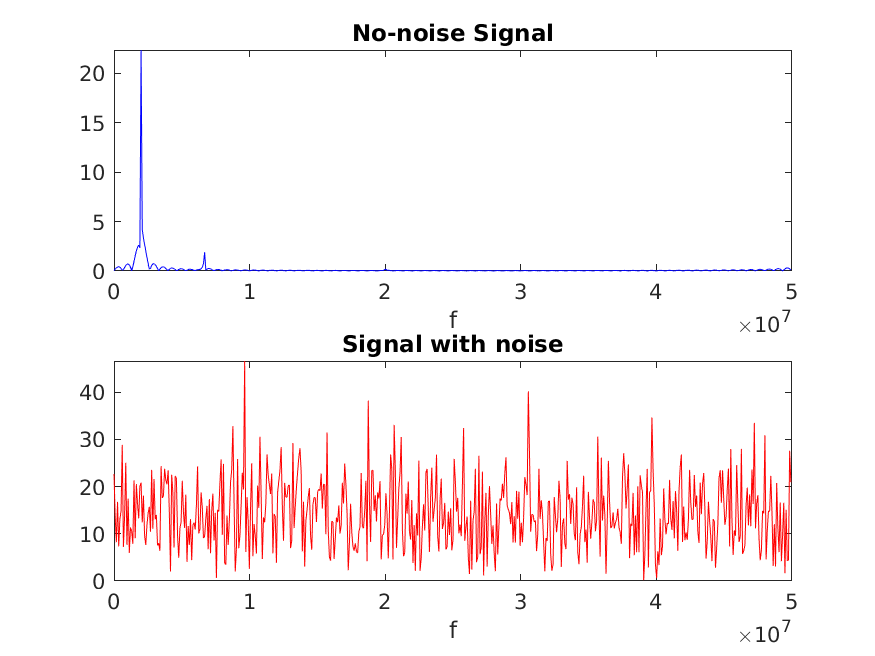
\includegraphics[width=0.7\textwidth]{images/signals_1.png}
      \captionof{figure}{Resulting Signals}
    \end{center}
\end{figure}

\begin{figure}[!hp]
    \begin{center}
      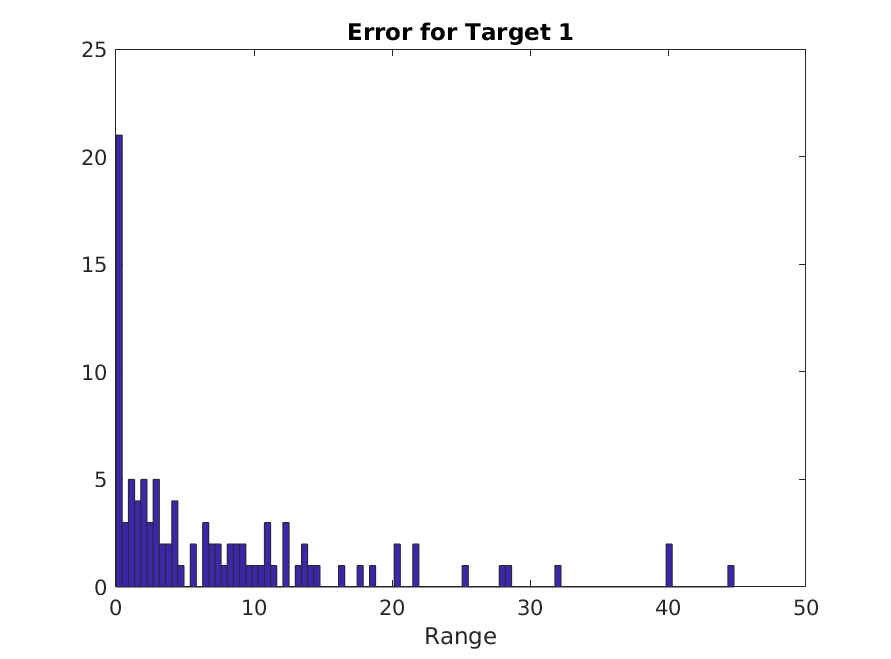
\includegraphics[width=0.7\textwidth]{images/hist_e1_1.png}
      \captionof{figure}{Histogram of the error for Target 1}
    \end{center}
\end{figure}

\begin{figure}[!hp]
    \begin{center}
      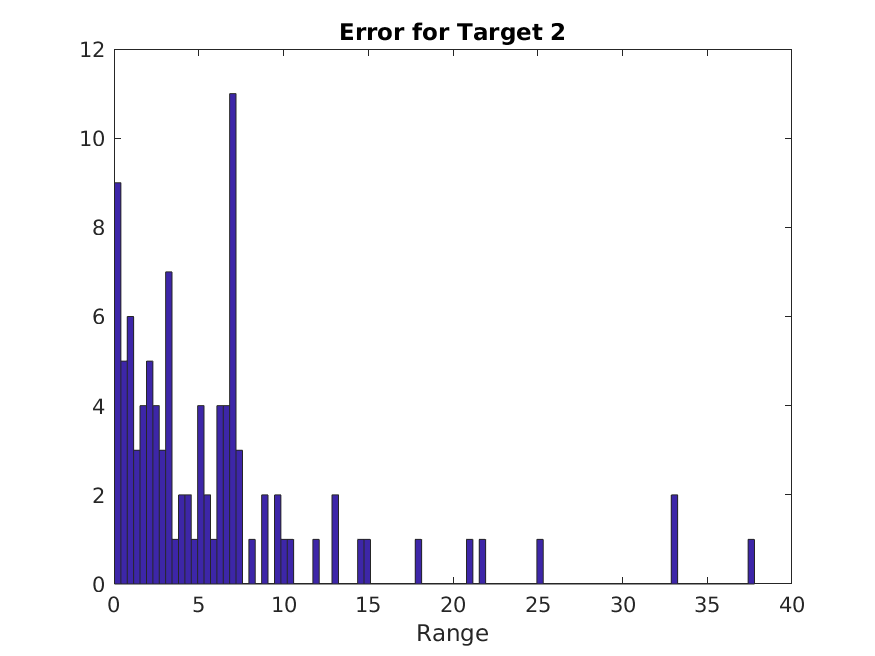
\includegraphics[width=0.7\textwidth]{images/hist_e2_1.png}
      \captionof{figure}{Histogram of the error for Target 2}
    \end{center}
\end{figure}

\begin{figure}[!hp]
    \begin{center}
      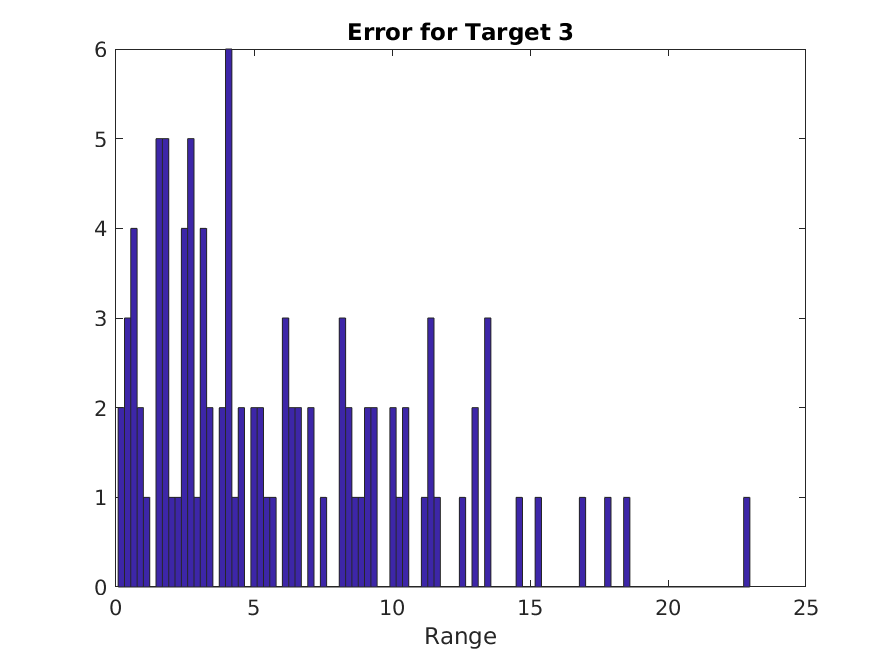
\includegraphics[width=0.7\textwidth]{images/hist_e3_1.png}
      \captionof{figure}{Histogram of the error for Target 3}
    \end{center}
\end{figure}

\newpage

\subsection{$SNR = 10$}

\begin{figure}[!hp]
    \begin{center}
      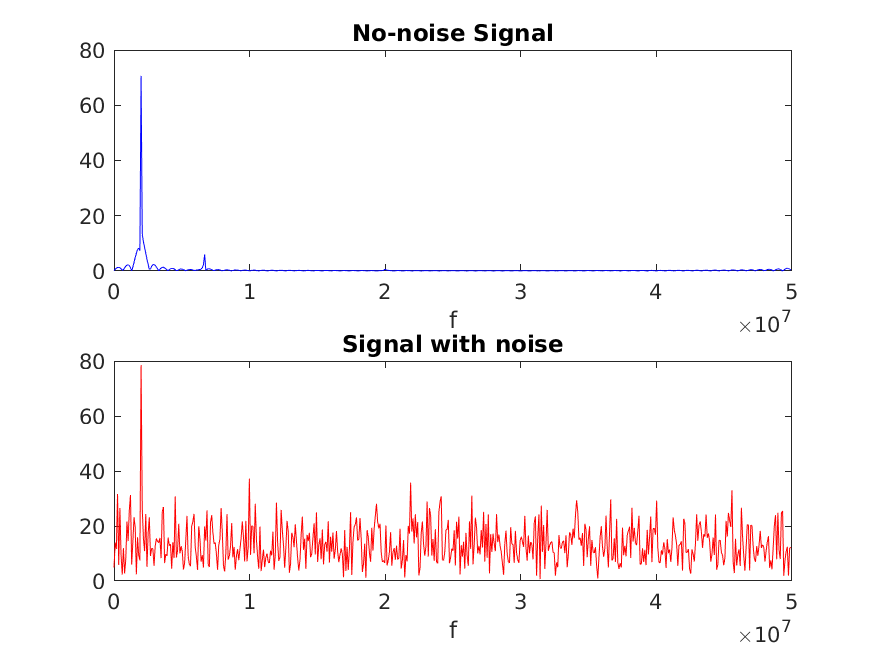
\includegraphics[width=0.7\textwidth]{images/signals_10.png}
      \captionof{figure}{Resulting Signals}
    \end{center}
\end{figure}

\begin{figure}[!hp]
    \begin{center}
      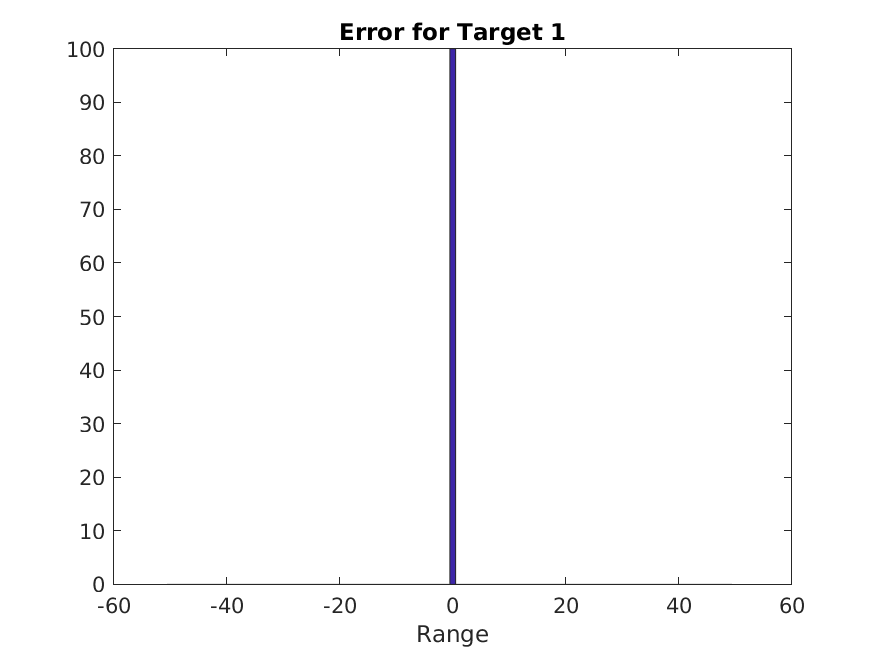
\includegraphics[width=0.7\textwidth]{images/hist_e1_10.png}
      \captionof{figure}{Histogram of the error for Target 1}
    \end{center}
\end{figure}

\begin{figure}[!hp]
    \begin{center}
      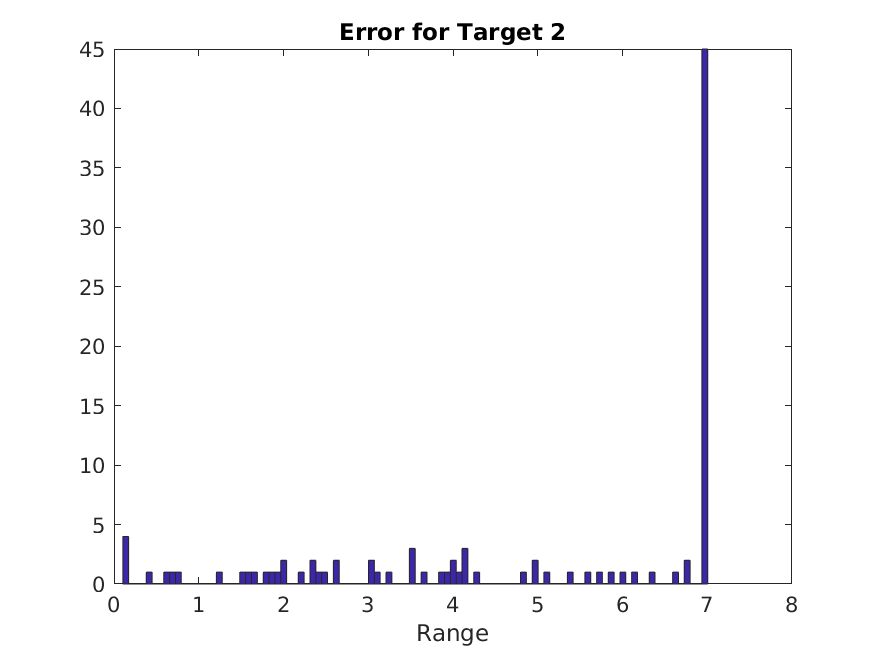
\includegraphics[width=0.7\textwidth]{images/hist_e2_10.png}
      \captionof{figure}{Histogram of the error for Target 2}
    \end{center}
\end{figure}

\begin{figure}[!hp]
    \begin{center}
      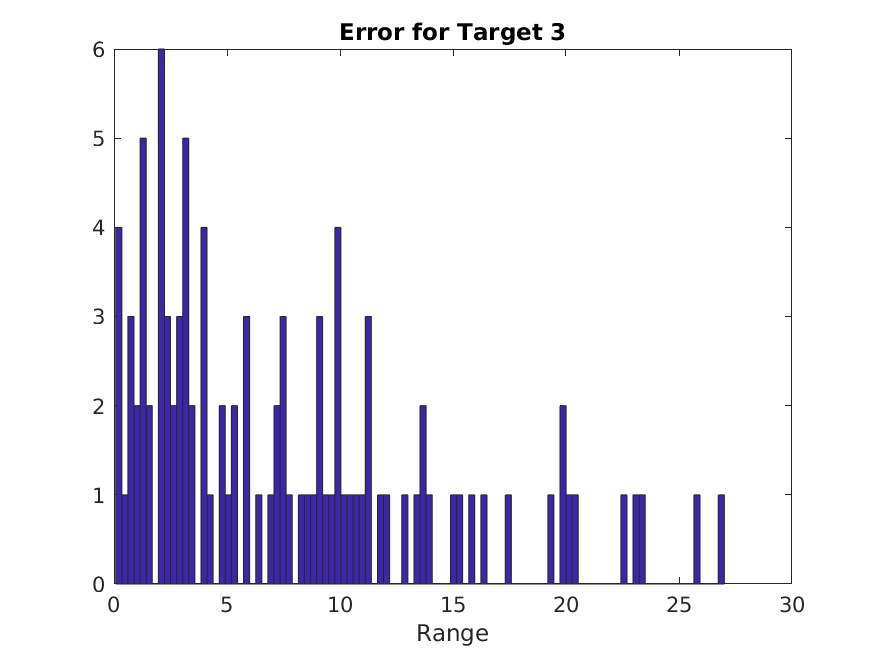
\includegraphics[width=0.7\textwidth]{images/hist_e3_10.png}
      \captionof{figure}{Histogram of the error for Target 3}
    \end{center}
\end{figure}

\newpage

\subsection{$SNR = 50$}

\begin{figure}[!hp]
    \begin{center}
      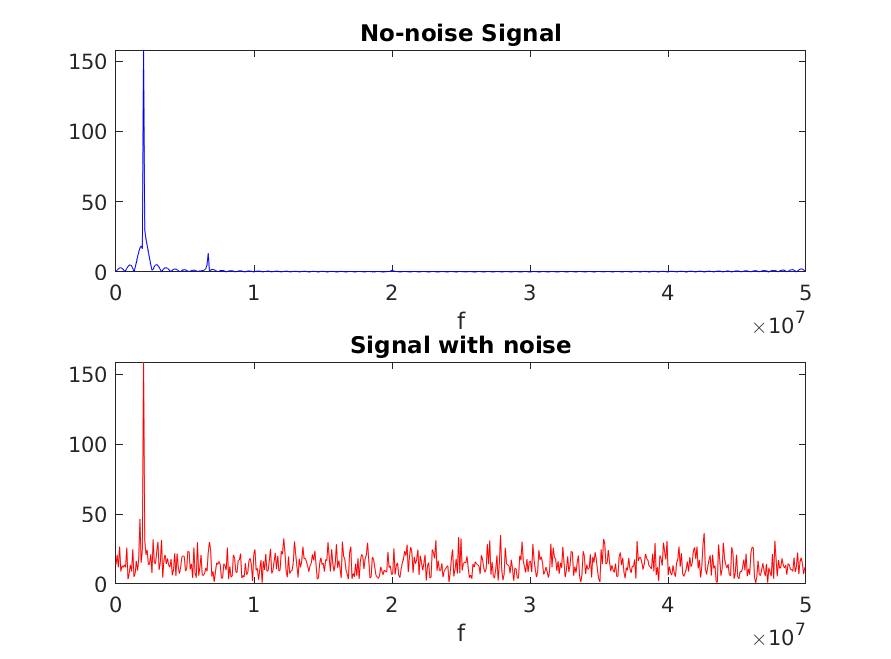
\includegraphics[width=0.7\textwidth]{images/signals_50.png}
      \captionof{figure}{Resulting Signals}
    \end{center}
\end{figure}

\begin{figure}[!hp]
    \begin{center}
      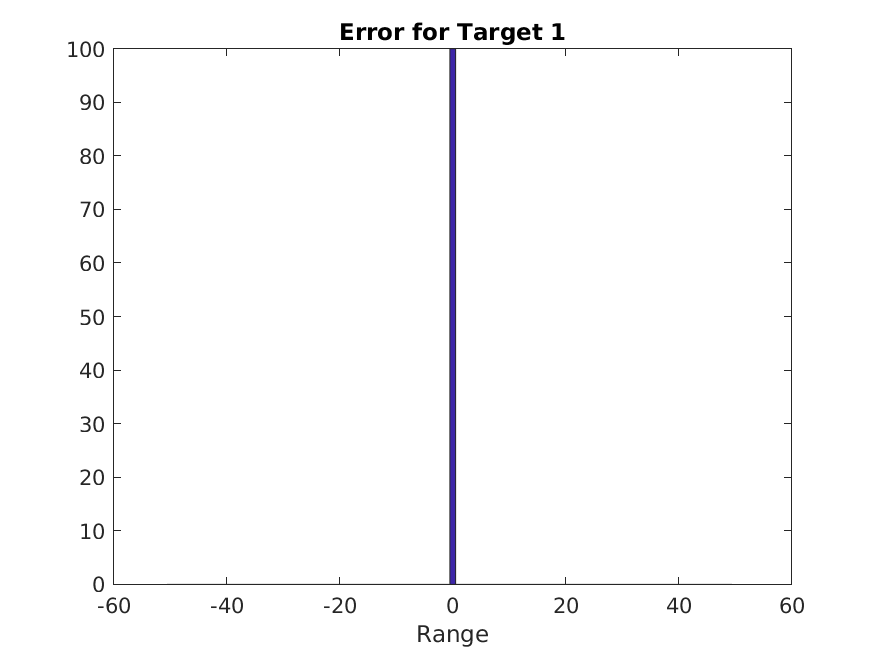
\includegraphics[width=0.7\textwidth]{images/hist_e1_50.png}
      \captionof{figure}{Histogram of the error for Target 1}
    \end{center}
\end{figure}

\begin{figure}[!hp]
    \begin{center}
      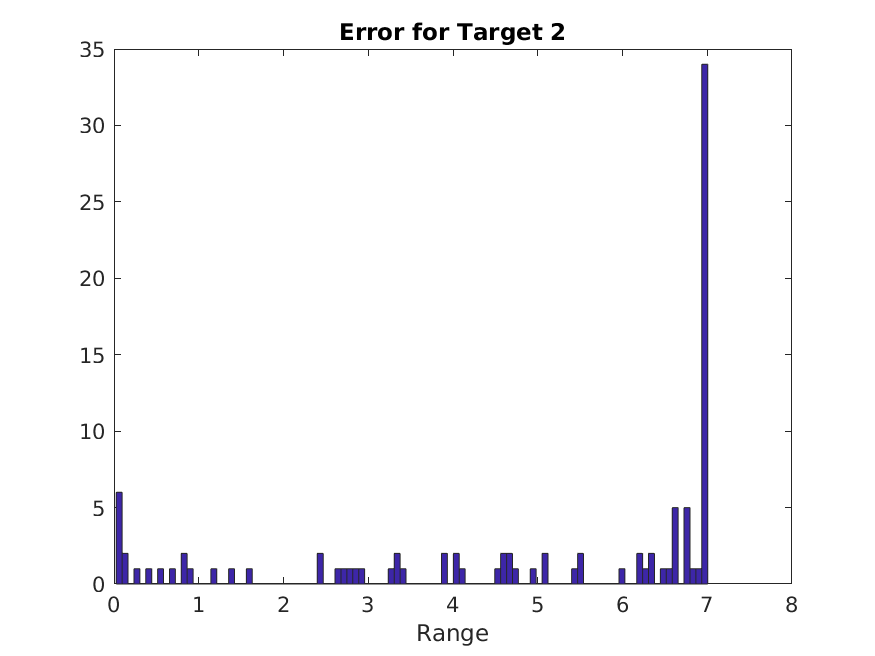
\includegraphics[width=0.7\textwidth]{images/hist_e2_50.png}
      \captionof{figure}{Histogram of the error for Target 2}
    \end{center}
\end{figure}

\begin{figure}[!hp]
    \begin{center}
      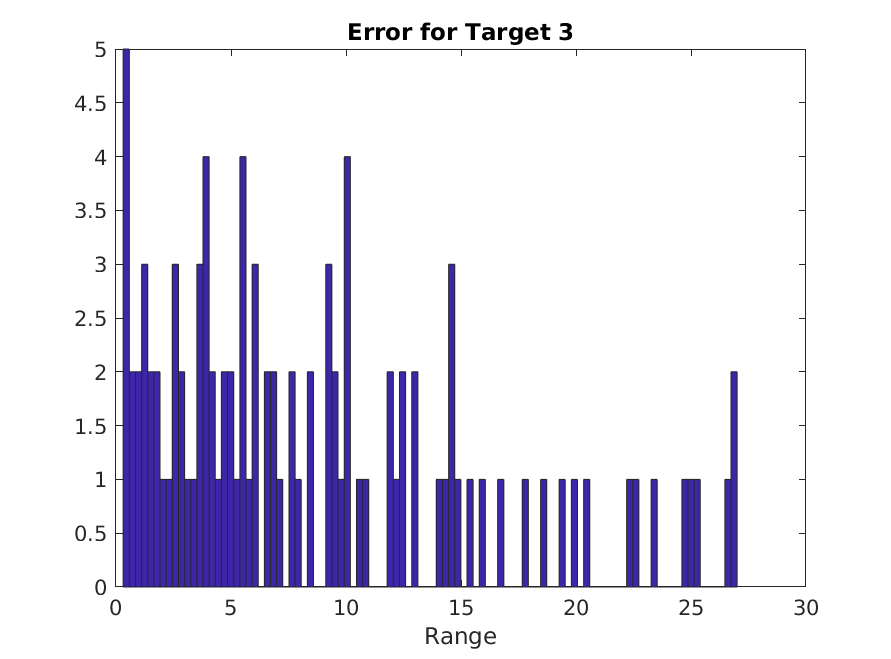
\includegraphics[width=0.7\textwidth]{images/hist_e3_50.png}
      \captionof{figure}{Histogram of the error for Target 3}
    \end{center}
\end{figure}

\newpage

\section{Analysis:}

As we can see, the error for target 1 is always smaller than for the other two
targets. This is due to the fact that the distance affects the clearness of the
signal squared, that is, multiplied by $\displaystyle\frac{1}{R^2}$. The error
for target 2 is quite high for $SNR = 1$, but it gets smaller the higher our
SNR is. Nevertheless, the error for target 3 is always very high compared to
the other two because $30m$ is a very long distance compared to $3m$ for
target 1, even if the SNR is 50.

\section{Conclusions:}

This lab was a good review of how receivers and transmitters work, and useful to
work with distances and other variables that have a huge impact on the signal.

The only problem I experienced with this lab is that I was not storing my error
vector correctly in the beginning so I had the same error for every iteration
according to my histogram. Once that was fixed, it was very smooth to continue
with all the calculations.

Unfortunately, due to the time of the quarter (dead week) I could not do the
optional part of the lab in time to hand it in. Nevertheless, I worked a bit
with it and I will study it before the final exam.

\vspace{4cm}

\end{document}
